% \documentclass[a4paper,10pt]{article}
\documentclass[review]{siamart}
\usepackage{url}
\usepackage{amssymb}
\usepackage{amsmath}
\usepackage{bm}
\usepackage{stmaryrd}
\usepackage{array}
\usepackage{empheq}
\usepackage{enumitem}
	\setlist{nosep} % or \setlist{noitemsep} to leave space around whole list
\usepackage{color}
\usepackage{showlabels}
\usepackage{adjustbox}
\usepackage{hyperref}
\hypersetup{
  colorlinks   = true, %Colours links instead of ugly boxes
  urlcolor     = blue, %Colour for external hyperlinks
  linkcolor    = blue, %Colour of internal links
  citecolor   = red %Colour of citations
}
\usepackage[numbers,sort]{natbib}
\usepackage{cleveref}

\newsiamremark{remark}{Remark}


% \newtheorem{lemma}{Lemma}
% \newtheorem{definition}{Definition}
% \newtheorem{theorem}{Theorem}
% \newtheorem{corollary}{Corollary}

\newcommand{\tcb}{\textcolor{blue}}
\newcommand{\tcp}{\textcolor{purple}}
\newcommand{\todo}[1]{\textcolor{red}{[TODO\@: #1]}}

\newcommand{\mdet}{\operatorname{det}}
\newcommand{\madj}{\operatorname{adj}}

% ------------------------------------------------------------------------------------ %
% ------------------------------------------------------------------------------------ %

\newcommand{\TheTitle}{IRK!}
\newcommand{\TheAuthors}{B.S. Southworth }
\headers{IRK!}{\TheAuthors}
\title{{\TheTitle}\thanks{This research was conducted ...
  }}

\author{%
  Ben~S.~Southworth
  \thanks{Department of Applied Mathematics,
          University of Colorado at Boulder
          (\email{ben.s.southworth@gmail.com}).}
}

\ifpdf%
\hypersetup{%
  pdftitle={\TheTitle},
  pdfauthor={\TheAuthors}
}
\fi

% ------------------------------------------------------------------------------------ %
% ------------------------------------------------------------------------------------ %

\begin{document}
\maketitle
\allowdisplaybreaks

\begin{abstract}

\end{abstract}


% ----------------------------------------------------------------------------------------------------------- %
% ----------------------------------------------------------------------------------------------------------- %
% ----------------------------------------------------------------------------------------------------------- %
\section{Introduction}

% ----------------------------------------------------------------------------------------------------------- %
% ----------------------------------------------------------------------------------------------------------- %
\subsection{Fully implicit Runge-Kutta}

Consider the method-of-lines approach to solving partial differential equations (PDEs),
where we discretize in space and arrive at a system of ODEs in time,
%
\begin{align}\label{eq:problem}
	M\mathbf{u}'(t) =  \mathcal{N}(\mathbf{u},t) \quad\text{in }(0,T], \quad \mathbf{u}(0) = \mathbf{u}_0,
\end{align}
%
where $M$ is a mass matrix, and $\mathcal{N}\in\mathbb{R}^{N\times N}$ a discrete, time-dependent, nonlinear
operator depending on $t$ and $\mathbf{u}$ (including potential forcing terms).
Then consider time propagation using an $s$-stage
Runge-Kutta scheme, characterized by the Butcher tableaux 
%
\begin{align*}
	\renewcommand\arraystretch{1.2}
	\begin{array}
	{c|c}
	\mathbf{c}_0 & A_0\\
	\hline
	& \mathbf{b}_0^T
	\end{array},
\end{align*}
%
with Runge-Kutta matrix $A_0 = (a_{ij})$, weight vector $\mathbf{b}_0^T = (b_1, \ldots, b_s)^T$, and 
nodes $\mathbf{c}_0 = (c_0, \ldots, c_s)$.

Runge-Kutta methods update the solution using a sum over stage vectors,
%
\begin{align*}
\mathbf{u}_{n+1} & = \mathbf{u}_n + \delta t \sum_{i=1}^s b_i\mathbf{k}_i, \\
M\mathbf{k}_i & = \mathcal{N}\left(\mathbf{u}_n + \delta t\sum_{j=1}^s a_{ij}\mathbf{k}_j, t_n+\delta tc_i\right).
\end{align*}
%
For nonlinear PDEs, $\mathcal{N}$ is linearized using, for example, a Newton or a Picard
linearization of the underlying PDE. Let us denote this linearization $\mathcal{L}\in\mathbb{R}^{N\times N}$
(or, in the case of a linear PDE, let $\mathcal{L} := \mathcal{N}$).
Expanding, solving for the stages $\mathbf{k}$ as each step in a nonlinear iteration, or
as the update to $\mathbf{u}$ for a linear PDE, can then be expressed as a block linear system,
%
\begin{align}\label{eq:k0}
\left( \begin{bmatrix} M  & & \mathbf{0} \\ & \ddots \\ \mathbf{0} & & M\end{bmatrix}
	- \delta t \begin{bmatrix} a_{11}\mathcal{L}_1 & ... & a_{1s}\mathcal{L}_1 \\
	\vdots & \ddots & \vdots \\ a_{s1}\mathcal{L}_s & ... & a_{ss} \mathcal{L}_s \end{bmatrix} \right)
	\begin{bmatrix} \mathbf{k}_1 \\ \vdots \\ \mathbf{k}_s \end{bmatrix} 
& = \begin{bmatrix} \mathbf{f}_1 \\ \vdots \\ \mathbf{f}_s \end{bmatrix}.
\end{align}
%

The difficulty in fully implicit Runge-Kutta methods (which we will denote IRK) lies in
solving the $Ns\times Ns$ block linear system in \eqref{eq:k0}. This paper focuses on the
parallel simulation of numerical PDEs, where $N$ is typically very large, on the order of
millions or billions, and $\mathcal{L}$ is highly ill-conditioned. In such cases, direct
solution techniques to solve \eqref{eq:k0} are not a viable option, and fast, parallel 
iterative methods must be used. However, IRK methods are rarely employed in practice due
to the difficulties of solving \eqref{eq:k0}. Even for relatively simple
parabolic PDEs where $\mathcal{L}$ is symmetric positive definite, \eqref{eq:k0}
instead yields a large nonsymmetric system with significant block coupling. For
nonsymmetric systems $\mathcal{L}$ that already have variable coupling, fast iterative
methods are even less likely to yield acceptable performance in solving \eqref{eq:k0}.

% TODO : add citations
Nevertheless, there are a number of desirable properties of IRK schemes, particularly
in terms of accuracy and stabillity. Practical alternatives to IRK schemes include
diagonally implicit Runge-Kutta methods (DIRK), where $A_0$ is lower triangular, or
singly implicit Runge Kutta methods (SIRK), where $A_0$ has exactly one positive real
eigenvalue. For such schemes, the solution of \eqref{eq:k0} only requires $s$ linear
solves of $M - \delta ta_{ii}\mathcal{L}_i$. Unfortunately, SIRK and DIRK schemes
suffer from stage-order one (stage-order two with one explicit stage), and for nonlinear
PDEs, it is typically the case that the global order of accuracy is limited to
$\approx \min\{ p, q+1\}$, for integration order $p$ and stage-order $q$. In addition
\todo{ref stability}. Thus, actually getting high-order accuracy with stiff PDEs
more-or-less requires the use of IRK methods.

A common approach for using IRK methods in practice is to assume $\mathcal{L}_i =
\mathcal{L}_j$ for all $i,j$, that is, $\mathcal{L}$ has no dependence on time. For
nonlinear problems, this corresponds to a simplified Newton method, where the Jacobian
is only evaluated at one time-point per time step (or also naturally arises for a
linear problem with no time-dependence in spatial differential components). This
yields a simplified form of \eqref{eq:k0} that can be expressed in Kronecker product
form,
%
\begin{align}\label{eq:kron1}
(I\otimes M - \delta t A_0\otimes \mathcal{L})\mathbf{k} & = \mathbf{f},
\end{align}
%
where $\mathcal{L}$ is a real-valued spatial operator or Jacobian independent of time.
Here, we revive some of the older Runge-Kutta work in the light of a changing
computational landscape, developing a new iterative approach to solve \eqref{eq:kron1}.
The new method effectively requires $s$ real-valued linear solves of matrices along the
lines of $\eta M - \delta t\mathcal{L}$, for some $\eta > 1$, and is easily implemented
using existing preconditioners and parallel software libraries. In addition, some of
the results generalize to the weaker scenario of commuting spatial operators,
$\mathcal{L}_i\mathcal{L}_j = \mathcal{L}_j\mathcal{L}_i$,
which provides a first step towards the fast solution of time-dependent IRK.

\tcb{ALso maybe useful in solving SDIRK because $\eta \gg a_{ij}$??}


\todo{outline sections}

% ----------------------------------------------------------------------------------------------------------- %
% ----------------------------------------------------------------------------------------------------------- %
\subsection{Why IRK and previous work}\label{sec:intro:prev}

% To avoid complex arithmetic, one can pose each complex
% system as a real $2\times 2$ block system,
% Because eigenvalues come in conjugate pairs, we will
% instead consider inverting conjugate pairs $(\overline{\lambda_i}I - \mathcal{L})^{-1}
% = \overline{(\lambda_iI - \mathcal{L})^{-1}}$, and thus the same solver/preconditioner
% could be used for conjugate pairs of eigenvalues \todo{cite}. However, this does not
% solve the underlying problem of constructing complex solvers/preconditioners in
% practice. 

The Kronecker product form (resulting from the assumption that $\mathcal{L}$ is independent of
time) allows for further simplifications. First proposed in \todo{Butcher77}, let $A_0$ have
Jordan normal form $A_0 = U_0L_0U_0^{-1}$, where $L_0$ is lower triangular, with eigenvalues
of $A_0$ on the diagonal and lower triangular entries corresponding to the (unit-valued)
Jordan blocks. Then \eqref{eq:kron1} is equivalent to the problem
%
\begin{align}\label{eq:kron2}
(U_0\otimes I)(I\otimes M - \delta t L_0\otimes \mathcal{L})(U_0^{-1}\otimes I)\mathbf{k} & = \mathbf{f},\\
(I\otimes M - \delta t L_0\otimes \mathcal{L})\hat{\mathbf{k}} & = \hat{\mathbf{f}},
\end{align}
%
where $\hat{\mathbf{f}} := (U_0^{-1}\otimes I)\mathbf{f}$ and
$\hat{\mathbf{k}} := (U_0^{-1}\otimes I)\mathbf{k}$. Note that computing the Jordan
decomposition of $A_0$ is typically of trivial computational expense compared to other
operations. The transformed system in \eqref{eq:kron2} can now be inverted by applying
a block diagonal or lower triangular solve, which only requires inverting the diagonal
blocks, $M - \delta_t(L_0)_{ii}\mathcal{L}$.

Transforming \eqref{eq:kron1} into \eqref{eq:kron2} reduces the solution of an $ns\times ns$
system of equations to solving $s$ linear systems of size $n\times n$. The downside is that the
IRK schemes with high accuracy and stability have primarily complex eigenvalues, in which case
the original real-valued system was transformed into a set of smaller complex systems (if the
original matrix $\mathcal{L}$ is complex, obviously complex eigenvalues are not a concern).
Complex eigenvalues introduce several difficulties. First, complex operations require several
times the floating-point operations to perform standard algebraic operations. Second, not
all preconditioners are well-developed for complex-valued matrices. Last, an important
practical concern is that not all software libraries support complex numbers. 

Published shortly after (and independently from) Butcher's result regarding Jordan normal
form \todo{cite}, Bickart developed a similar result \todo{cite}. If we define $Q_s(x)$ as the characteristic
polynomial of $A_0$, then the inverse of \eqref{eq:kron1} can be computed via some matrix-vector
multiplications and the action of $Q_s(\mathcal{L})^{-1}$ \todo{cite}. This is similar in principle to
Butcher's result, as in practice one could invert $Q_s(\mathcal{L})$ by inverting 
each term in the factored polynomial, $(\mu_1 I-\mathcal{L})^{-1}$,
$(\mu_2 I-\mathcal{L})^{-1}$, ..., for eigenvalues $\{\mu_i\}_{i=1}^s$ of $A_0$.
Although Bickart's paper received less attention than Butcher's over time (currently $2.5\times$
less citations), the polynomial form provides a more natural way to handle complex eigenvalues,
particularly in the modern high-performance computing landscape, where direct LU inverses
are rare and most linear systems are solved via preconditioning and/or Krylov methods. 

\todo{Fix discussion on Bickart's result, work out what he actually did carefully.}

% Simplified newton scheme uses fixed Jacobian for all stages
% Single step Newton (Cooper (83/90), Gonzales-Pinto (95/97)
% ---------------- ODEs and LU ---------------- %
Butcher (76), Bickart (77)
\begin{itemize}
	\item Uses tensor product structure, gets Jordan normal form of Butcher matrix A. Reformulates
	problem as block subdiagonal, with diagonal blocks $I - h\lambda J$, for Jacobian $J$, time step $h$,
	and eigenvalue $\lambda$ of $A$ (are we sure not $A^{-1}$??).
	\item Must solve for complex eigenvalues. This is not desirable. 
	\item Bickart uses polynomial form, closer to what I look at. Originally based on Tensor product
	result from Jameson (68)
\end{itemize}

Varah (79):
\begin{itemize}
	\item Much better description of Butcher's method. Transforms coordinate system of Jacobian tensor.
	Still relies on this tensor structure to do said transformation. 
	\item Transforms Jacobian to Hessenberg form to avoid repeated action computing LU of a shifted 
	Jacobian.
\end{itemize}

Burrage (82):
\begin{itemize}
	\item Look at stability of DIRK and SIRK methods, which have one eigenvalue and are more amenable
	to development by Butcher. 
\end{itemize}

Orel (91):
\begin{itemize}
	\item Looks at RK methods w/ real eigenvalues. Turns out best approximation to exponential is
	obtained by having all eigenvalues equal (SIRK/SDIRK methods). SIRK methods offer some advantages over SDIRK methods, but lack the favorable stabillity an accuracy of IRK methods. 
\end{itemize}

Cooper:
\begin{itemize}
	\item (83,90,93): develops single Newton scheme using SOR or various matrix splittings,
	applied to ODEs. This is a single-step
	Newton method, where the actual Jacobian solve is replaced with an SOR iteration. Here, Butcher
	matrix A is replaced with an approximate matrix with one positive real eigenvalue. 
\end{itemize}

Pinto:
\begin{itemize}
	\item (95) Mostly ODEs, do consider 1d-space-1d-time burgers on a very small grid. 
	\item (96) additional iteration of single Newton, makes it quasi-Newton like. 
	\item (01) Analysis of single Newton (SOR) w/ simplified Newton for higer order. 
\end{itemize}


Butcher (2000):
\begin{itemize}
	\item Develops ESDIRK schemes w/ higher stage order and stiff accuracy than traditional
	SIRK/DIRK schemes. Based on using iniital explicit stage, moves RK abscissae.
\end{itemize}


Brugano (2014) and Antonana (2018)
\begin{itemize}
	\item New splitting and IRK techniques for Hamiltonian problems where conservation is
	important. Used for ODEs. 
\end{itemize}


% ---------------- PDEs ---------------- %

\begin{itemize}
	\item One obvious drawback -- even if spatial operator/Jacobian is SPD, IRK system is
	nonsymmetric.
\end{itemize}

Lay (2000)
\begin{itemize}
	\item 
\end{itemize}

Van Lent (2004)
\begin{itemize}
	\item Multigrid for IRK?
\end{itemize}

Staff \& Mardal (2006)
\begin{itemize}
	\item One of first paper to consider preconditioning the fully implicit RK system.
	Use block Jacobi and block lower triangular preconditioners for the diffusion equation.
	Use multigrid V-cycles and full Newton time-dependent Jacobian. Upper triangular is
	bad compared to block Jacobi and lower triangular (this has appeared elsewhere in
	literature -- $A_0$ is dominant in lower triangular part -- Crout factorization
	in I think Messina or Van der Houwen; comes up again in Brugano (2015)).
\end{itemize}
Mardal (2007)
\begin{itemize}
	\item Analyze block-diagonal preconditioners in a Sobolev setting, demonstrate
	conditioning of the preconditioned operator to be optimal in the independent of
	$h$ sense. Use multigrid w/ diffusion as example. 
\end{itemize}
Nilssen (2011)
\begin{itemize}
	\item Analogous to above, Sobolev analysis for block-diagonal preconditioning
	applied to the bidomain equations.
\end{itemize}

Xie (2011)
\begin{itemize}
	\item Proposes a modified simplified Newton for the time-dependent cast, where the Jacobian is
	formed based on a least squares approximation to the true RK coefficients, evaluating all entries
	at a single time point. In example problems, modified Jacobian typically converged faster
	than simplified (evaluated at previous time step), up to 2x less iterations/time. 
\end{itemize}

Hao Chen:
\begin{itemize}
	\item (2014) Develops a splitting iterative method to precondition IRK matrices, similar to ADI schemes.
	Proves that for definite spatial operators and Butcher matrices (that is, eignvalues have positive
	or negative real parts), $\rho(T) < 1$, where $T$ is the fixed-point iteration matrix. Look at 
	diffusion equation with IRK and BVMs.
	\item (2016) Analogous to above, extended to wave equation.
\end{itemize}

Pazner
\begin{itemize}
	\item
\end{itemize}



% ----------------------------------------------------------------------------------------------------------- %
% ----------------------------------------------------------------------------------------------------------- %
% ----------------------------------------------------------------------------------------------------------- %
\section{Fast parallel solvers for IRK}

The RK stage system in \eqref{eq:k0} can be reformulated as \todo{cite Will}
%
\begin{align}\label{eq:keq}
\left( A_0^{-1}\otimes M - \delta t \begin{bmatrix} \mathcal{L}_1  & \\ & \ddots \\ && \mathcal{L}_s\end{bmatrix}\right)
	(A_0\otimes I)	\begin{bmatrix} \mathbf{k}_1 \\ \vdots \\ \mathbf{k}_s \end{bmatrix} 
& = \begin{bmatrix} \mathbf{f}_1 \\ \vdots \\ \mathbf{f}_s \end{bmatrix}.
\end{align}
%
For ease of notation, let us scale both sides of the system by a block-diagonal mass matrix 
and, excusing the slight abuse of notation, let $\mathcal{L}_i \mapsto \delta t M^{-1}\mathcal{L}_i$,
$i=1,..,s$ \tcp{[Maybe we should write $\hat{\cal L}_i \coloneqq \delta t M^{-1}\mathcal{L}_i$? Since it's a bit confusing/misleading: Applying the action of ${\cal L}$ is simpler and less expensive than $\hat{\cal L}$, which involves a mass matrix solve. Also, I'm not sure that all properties of ${\cal L}_i$ extend to $\hat{\cal L}_i$, like commutativity?]}. Note the time step $\delta t$ for the given Runge-Kutta step is now included in $\mathcal{L}_i$. Now let $\alpha_{ij}$ denote the $ij$-element of $A_0^{-1}$ (assuming $A_0$ is
invertible). Then, solving \eqref{eq:k0} can be effectively reduced to inverting the operator
%
\begin{align}\nonumber
\mathcal{M}_s & := A_0^{-1}\otimes I - \begin{bmatrix} \mathcal{L}_1  & \\ & \ddots \\ && \mathcal{L}_s\end{bmatrix} \\
& = \begin{bmatrix} \alpha_{11}I - \mathcal{L}_1 & \alpha_{12}I & ... & \alpha_{1s}I \\
	\alpha_{21}I & \alpha_{22}I - \mathcal{L}_2 & & \alpha_{2s}I \\
	\ddots & & \ddots & \vdots \\ \alpha_{s1}I & ... & \alpha_{s(s-1)}I & \alpha_{ss}I - \mathcal{L}_s \end{bmatrix}.
	\label{eq:k1}
\end{align}
%

Note, there are a number of methods with one explicit stage preceded or followed by several
fully implicit and coupled stages. In such cases, $A_0$ is
not invertible, but the explicit stage can be eliminated from the system (by doing an explicit
time step). The remaining operator can then be reformulated as above, and the inverse that
must be applied takes the form of \eqref{eq:k1} but based on a principle submatrix of $A_0$.

% ----------------------------------------------------------------------------------------------------------- %
% ----------------------------------------------------------------------------------------------------------- %
\subsection{An inverse and update for commuting operators}\label{sec:solve:inv}

This section introduces a result similar to Bickart's but generalized to hold for commuting
operators. If $\mathcal{L}_i=\mathcal{L}_j$ for all $i,j$, we show that the inverse of
\eqref{eq:k1} can be expressed in terms of $P_s(\mathcal{L})^{-1}$, where $P_s(\mathcal{L})$
is the characteristic polynomial of $A_0^{-1}$.

%
\begin{lemma}\label{lem:inv}
Let $\alpha_{ij}$ denote the $(i,j)$th entry of $A_0^{-1}$ and assume $\{\mathcal{L}_i\}_{i=1}^s$
are commuting operators\footnote{\tcp{Does the mass matrix stop this from happening though? Because if the true spatial discretizations $\{\mathcal{L}_i\}_{i=1}^s$ commute, how likely is it that the mass-matrix scaled operators $\{ \hat{\cal L}_i \}_{i=1}^s = \{\delta t M^{-1} \mathcal{L}_i\}_{i=1}^s$ commute? Wouldn't this mean that $M^{-1}$ has to commute with all ${\cal L}_i$?}}. Define $\mathcal{M}_s$
% \begin{align*}
% \mathcal{M}_s := \begin{bmatrix} \alpha_{11}I - \mathcal{L}_1 & \alpha_{12}I & ... & \alpha_{1s}I \\
% 	\alpha_{21}I & \alpha_{22}I - \mathcal{L}_2 & & \alpha_{2s}I \\
% 	\ddots & & \ddots & \vdots \\ \alpha_{s1}I & ... & \alpha_{s(s-1)}I & \alpha_{ss}I - \mathcal{L}_s \end{bmatrix},
% \end{align*}
as in \eqref{eq:kron1}  \tcp{[Do you mean  \eqref{eq:k1}?]}.
Let det$(\mathcal{M}_s)$ be the determinant of $\mathcal{M}_s$ (in this case a block-diagonal
matrix\footnote{\tcp{What does it mean for a determinant to be a block matrix, though? Isn't a determinant always a scalar? This relates to my long comment below.}}) and let adj$(\mathcal{M}_s)$ be the adjugate of $\mathcal{M}_s$. Then, $\mathcal{M}_s$
is invertible if and only if $\mathcal{D}_s$ is invertible\footnote{\tcp{What is $\mathcal{D}_s$?}}, and\footnote{\tcp{In this equation, should this be ``det$(\mathcal{M}_s)$'' rather than ``det$({M}_s)$'', and also in all the places following this equation where you have ``det$({M}_s)$''?}}
\begin{align*}
\mathcal{M}_s^{-1} = \textnormal{det}({M}_s)^{-1}\textnormal{adj}(\mathcal{M}_s).
\end{align*}{}

Now, suppose $\mathcal{L}_i = \mathcal{L}_j$ for all $i,j$, and let $P_s(x)$ be the
characteristic polynomial of $A_0^{-1}$. Then,
\begin{align*}
\mathcal{M}_s^{-1} = \textnormal{diag}(P_s(\mathcal{L})^{-1})\textnormal{adj}(\mathcal{M}_s),
\end{align*}
where ``diag'' indicates a block diagonal matrix, with diagonal blocks given by $P_s(\mathcal{L})^{-1}$.
\end{lemma}
%
\begin{proof}
Notice in \eqref{eq:k1} that if $\mathcal{L}_i$ and $\mathcal{L}_j$ commute for all $i,j$,
then $\mathcal{M}_s$ is a matrix over the commutative ring of linear combinations
of $I$ and $\{\mathcal{L}_i\}$. Let adj$(\mathcal{M}_s)$ denote the matrix adjugate. A
classical result in matrix analysis then tells us that
%
\begin{align*} 
\textnormal{adj}(\mathcal{M}_s)\mathcal{M}_s = \mathcal{M}_s\textnormal{adj}(\mathcal{M}_s)
	= \textnormal{det}(\mathcal{M}_s)I.
\end{align*}
%
Moreover, $\mathcal{M}_s$ is invertible if and only if if the determinant of $\mathcal{M}_s$
is invertible, in which case $\mathcal{M}_s^{-1} := $ det$(\mathcal{M}_s)^{-1}$adj$(\mathcal{M}_s)$.
\todo{Need citations!}
For the case of time-independent operators ($\mathcal{L}_i=\mathcal{L}_j$), notice that
$\mathcal{M}_s$ takes the form $A_0^{-1} - \mathcal{L}I$ over the commutative ring defined
above. Analogous to a scalar matrix, the determinant of $A_0^{-1} - \mathcal{L}I$ is the
characteristic polynomial of $A_0^{-1}$ evaluated at $\mathcal{L}$.
\end{proof}
%

\tcp{
I'm confused... I suspect this stems from the fact I don't really know (lack the background) what it means  that ${\cal M}_s$ is defined over a  ``commutative ring'' and what this allows you to do/what makes sense in terms of computing its inverse.
To clarify, do you mean that if we have the characteristic polynomial of $A_0^{-1}$, $P_s \colon \mathbb{C} \to \mathbb{C}$,
\[
P_s(z) = \det(A_0^{-1} - z I) = \prod_{k = 1}^s (\lambda_k - z), \quad \{\lambda\} {\rm \, the\, eigenvalues\, of\, }A_0^{-1},
\] 
and the matrix, ${\cal Q} \colon \mathbb{R} \to \mathbb{R}^{s \times s}$,
\[
\mathcal{Q}(z) = {\rm adj}(A_{0}^{-1} - zI) \in \mathbb{R}^{s \times s}, \quad {\rm with\, entries} \quad [\mathcal{Q}(z)]_{ij} = q_{ij}(z) \in \mathbb{R}.
\] 
Then, if we generalize these functions to take matrix-valued arguments (in the first by letting $\lambda_k \mapsto \lambda_k I$, and in the second by allowing each matrix element $q_{ij}(z)$ to be matrix valued) we can write the inverse of ${\cal M}_s$ as 
\begin{align*}
\mathcal{M}_s^{-1} 
&= \underbrace{\left( I_s \otimes \prod_{k = 1}^s (\lambda_k I - {\cal L}) \right)^{-1}}_{\neq \det({\cal M}_s)^{-1}?}
\underbrace{\begin{bmatrix}
q_{11} ({\cal L}) & \cdots & q_{1s}({\cal L}) \\
\vdots & \cdots & \vdots \\
q_{s1} ({\cal L}) & \cdots & q_{ss}({\cal L}) 
\end{bmatrix}}_{\neq {\rm adj}({\cal M}_s)?}.
\end{align*}
For example, when you say the ``determinant'' of $A_0^{-1} - {\cal L} I$, you mean the matrix $  I_s \otimes \prod_{k = 1}^s (\lambda_k I - {\cal L}) $ (or maybe even just $\prod_{k = 1}^s (\lambda_k I - {\cal L})$)? But this is not a determinant because it's a matrix and not a scalar? You cannot do $\det(A - z I)$ for $z$ a matrix, i.e., the characteristic polynomial of $A$ is not defined for matrix-valued inputs (e.g., what is $\lambda_k - {X}$ for some matrix $X$)? This is like the matrix $A_0^{-1} - {\cal L}I$ above, how does this matrix make sense?}\\

\tcp{
Does ${\cal M}_s$ being defined over a commutative ring just mean that it's a matrix whose elements are closed under addition/multiplication (i.e., they're from a commutative ring)? E.g., ${\cal M}_s$ being defined over a commutative ring of linear combinations of $I$ and ${\cal L}$ means that it's a matrix whose elements are given by linear combinations of $I$ and ${\cal L}$? And this fact somehow means we can generalize the definition of the determinant and adjugate from working with scalar matrix elements (which themselves come from a commutative ring) to matrix elements that are actually matrices from a commutative ring? So it's basically like what's described here for the determinant (\url{https://en.wikipedia.org/wiki/Determinant\#Square\_matrices\_over\_commutative\_rings\_and\_abstract\_properties}, but I  don't really understand the details...)?
}

\tcp{Anyways, if what I say above is kind of right, I don't understand the notation/how you distinguish between these operators and their generalizations (or don't you?). For example, I think the determinant of ${\cal M}_s$ is actually
\begin{align*}
\det {\cal M}_s \overset{?}{=} \det \prod_{k = 1}^s (\lambda_k I - {\cal L}),
\end{align*}
and 
\begin{align*}
{\rm det}_{\rm g} {\cal M}_s = \prod_{k = 1}^s (\lambda_k I - {\cal L})
\end{align*}
is like a generalized determinant of ${\cal M}_s$?
Similarly, the adjugate of ${\cal M}_s$ is
\begin{align*}
{\rm adj\,} {\cal M}_s \overset{?}{=} {\rm adj\,} 
\begin{bmatrix}
q_{11} ({\cal L}) & \cdots & q_{1s}({\cal L}) \\
\vdots & \cdots & \vdots \\
q_{s1} ({\cal L}) & \cdots & q_{ss}({\cal L}) 
\end{bmatrix},
\end{align*}
and 
\begin{align*}
{\rm adj}_{\rm g} = \begin{bmatrix}
q_{11} ({\cal L}) & \cdots & q_{1s}({\cal L}) \\
\vdots & \cdots & \vdots \\
q_{s1} ({\cal L}) & \cdots & q_{ss}({\cal L}) 
\end{bmatrix}
\end{align*}
is the generalized adjugate? Hmm, but adjugate relation doesn't quite hold in the MATLAB code I wrote... And from what you have above, I'm guessing that we can write the inverse of ${\cal M}$ using the generalized operators (except we need to do diag of the generalized determinant)?
}

Returning to \eqref{eq:keq}, we can express the direct solution for the set of all
stage vectors ${\mathbf{k}} = [\mathbf{k}_1; ...; \mathbf{k}_s]$ as
%
\begin{align*}
\mathbf{k} &:= \textnormal{det}({M}_s)^{-1}
	(A_0^{-1}\otimes I)\textnormal{adj}(\mathcal{M}_s)\mathbf{f},
\end{align*}
%
where $\mathbf{f} = [\mathbf{f}_1; ...; \mathbf{f}_s]$ (note that
$A_0\otimes I$ commutes with $\textnormal{det}({M}_s)^{-1}$). Excusing the slight
abuse in notation, let $\textnormal{det}({M}_s)^{-1}$ now denote just the diagonal
block (rather than a block-diagonal matrix). The Runge-Kutta update is then given by
%
\begin{align}\nonumber
\mathbf{u}_{n+1} & = \mathbf{u}_n + \delta t\sum_{i=1}^s b_i{\mathbf{k}}_i \\
& = \mathbf{u}_n + \delta t\textnormal{det}({M}_s)^{-1}
	(\mathbf{b}_0^TA_0^{-1}\otimes I)\textnormal{adj}(\mathcal{M}_s)\mathbf{f}.\label{eq:update}
\end{align}
%

The adjugate simply consists of linear combinations of $I$ and $\mathcal{L}$, and an
analytical form can be derived for an arbitrary $s\times s$ matrix, where $s\sim\mathcal{O}(1)$.
Computing this operator analytically is easiest using a computer algebra program
such as Mathematica. Applying its action will consist of some set of vector summations
and matrix-vector multiplications. In particular, the diagonal elements of
$\textnormal{adj}(\mathcal{M}_s)$ are monic polynomials in $\mathcal{L}$ of degree
$s-1$ (or linear combinations of comparable degree if $\mathcal{L}_i\neq\mathcal{L}_j$)
and off-diagonal terms are polynomials in $\mathcal{L}$ of degree $s-2$. 

Returning to \eqref{eq:update}, we consider two cases. First, if a given Runge-Kutta
scheme is stiffly accurate, then $\mathbf{b}_0^TA_0^{-1} = [0,...,0,1]$. This yields
the nice simplification that computing the update in \eqref{eq:update} only requires
applying the last row of $\textnormal{adj}(\mathcal{M}_s)$ to $\mathbf{f}$ (in a
dot product sense) and applying $\textnormal{det}({M}_s)^{-1}$ to the result. From
the discussion above regarding the adjugate structure, applying the last row of
$\textnormal{adj}(\mathcal{M}_s)$ requires $(s-2)(s-1) + (s-1) = (s-1)^2$ matrix-vector
multiplications. Because this only happens once, followed by the linear solve(s),
these multiplications are typically of relatively marginal cost.

In the more general case of non stiffly accurate (e.g., Gauss methods), one can
obtain (again using, e.g., Mathematica) an analytical form for
$(\mathbf{b}_0^TA_0^{-1}\otimes I)\textnormal{adj}(\mathcal{M}_s)$. Each element in
this matrix consists of polynomials in $\mathcal{L}$ of degree $s-1$ (although
typically not monic). Compared with stiffly accurate schemes, this now requires 
$(s-1)s$ matrix-vector multiplications, which is $s-1$ more than for stiffly
accurate schemes, but still typically of marginal overall computational cost. 

% ----------------------------------------------------------------------------------------------------------- %
% ----------------------------------------------------------------------------------------------------------- %
\subsection{Stability and the method of lines}

{\color{blue}
\begin{itemize}

\item A necessary condition for stable time-propagation is that eigenvalues of $\mathcal{L}$
lie in the region of stability for the given RK scheme. For virtually all implicit RK schemes,
this means that eigenvalues of $\mathcal{L}$ must have negative real part, or real part
$\gg 0$. It is rare for operators representing a differential discretization to be split
with a set of negative definite eigenvalues and a set of eigenvalues with real part $\gg 0$,
so for our purposes assume $\mathcal{L}$ has eigenvalues with negative real part.

\item Just eigenvalues is not strong enough for our analysis or stability. Need to look
into literature. Would be nice if it was related to numerical range/field of values, because
that is what our analysis is based on. Ideally, something along the lines of $\mathcal{L}$ 
has a non-positive field of values for stability? 
\end{itemize}
}


% ----------------------------------------------------------------------------------------------------------- %
% ----------------------------------------------------------------------------------------------------------- %
\subsection{Preconditioning by conjugate pairs}

Following the discussion and algorithm developed in \Cref{sec:solve:inv}, the key
outstanding point is inverting $\textnormal{det}({M}_s)^{-1}$. Moving forward, we
restrict our attention to the case $\mathcal{L}_i = \mathcal{L}_j$ for all $i,j$,
in which case $\textnormal{det}({M}_s)^{-1} = P_s(\mathcal{L})^{-1}$, where
$P_s(x)$ is the characteristic polynomial of $A_0^{-1}$ (see \Cref{lem:inv}).

In contrast to some of the original work on solving IRK systems, where LU factorizations
were the dominant cost and system sizes relatively small \todo{cite}, explicitly forming and inverting
$P_s(\mathcal{L})$ for numerical PDEs is typically not a viable option in high-performance
simulation on modern computing architectures. Instead, by computing the eigenvalues
$\{\lambda_i\}$ of $A_0^{-1}$, we can express $P_s(\mathcal{L})$ in a factored form, 
%
\begin{align}\label{eq:fac}
P_s(\mathcal{L}) = \prod_{i=1}^s (\lambda_i I - \mathcal{L}),
\end{align}
%
and its inverse can then be computed by successive applications of $(\lambda_iI - \mathcal{L})^{-1}$,
for $i=1,...,s$. As discussed previously, eigenvalues of $A_0$ and $A_0^{-1}$ will often be
complex, making the inverse of individual factors $(\lambda_iI - \mathcal{L})^{-1}$ more
difficult and often not practical. 

Here, we propose combining pairs of conjugate eigenvalues into quadratic polynomials
that we must precondition, which take the form 
%
\begin{align}\label{eq:imag1}
((\eta + i\beta)I - \mathcal{L})((\eta - i\beta)I - \mathcal{L}) =
	(\eta^2+\beta^2)I - 2\eta \mathcal{L} + \mathcal{L}^2.
\end{align}
%
In practice, we typically do not want to directly form or precondition a quadratic
operator like \eqref{eq:imag1}. For example, a discretization of diffusion is typically 
conditioned like $1/h^2$ for mesh spacing $h$ (worse for high-order discretizations),
so considering $\mathcal{L}^2$ directly results in conditioning $\sim\mathcal{O}(1/h^4)$.
Moreover, many fast parallel methods such as multigrid are not well-suited for solving
a polynomial in $\mathcal{L}$. The point of \eqref{eq:imag1} is that by considering
conjugate pairs of eigenvalues, the resulting operator is real-valued. Thus, consider
preconditioning \eqref{eq:imag1} with the inverse of the real-valued quadratic polynomial,
$(\eta I - \mathcal{L})(\eta I - \mathcal{L})$. Expanding, the preconditioned operator
takes the form
%
\begin{align}\nonumber
\mathcal{P}_A & := (\eta I - \mathcal{L})^{-2}\left[(\eta^2+\beta^2)I - 2\eta \mathcal{L} + \mathcal{L}^2\right] \\
&\hspace{5ex} = I + \beta^2(\eta I - \mathcal{L})^{-2}
= I + \frac{\beta^2}{\eta^2}\left(I - \tfrac{1}{\eta}\mathcal{L}\right)^{-2}.\label{eq:prec1}
\end{align}
%

It turns out, by assumptions on $\mathcal{L}$ that yield a stable time-propagation scheme,
the preconditioned operator in \eqref{eq:prec1} is very well-conditioned. 
\Cref{th:fov} analyzes the field-of-values of $\mathcal{P}_A$, denoted $W(\mathcal{P}_A)$,
as a measure of the preconditioning, and \Cref{cor:gmres} extends this preconditioning to
prove fast convergence of GMRES. 

%
\begin{theorem}\label{th:fov}
Assume that $\eta > 0$ and the symmetric part of $\mathcal{L}$ satisfies
$(\mathcal{L}+\mathcal{L}^T)/2 \leq 0$. Let $\mathcal{P}_A$ denote the preconditioned
operator, where $((\eta + i\beta)I - \mathcal{L})((\eta - i\beta)I - \mathcal{L})$ is
preconditioned with $(\eta I - \mathcal{L})^{-2}$. Then $W(\mathcal{P}_A)$ is bounded
by $\Omega$ as shown in \Cref{fig:bound}.
\begin{figure}[h!]
\centering
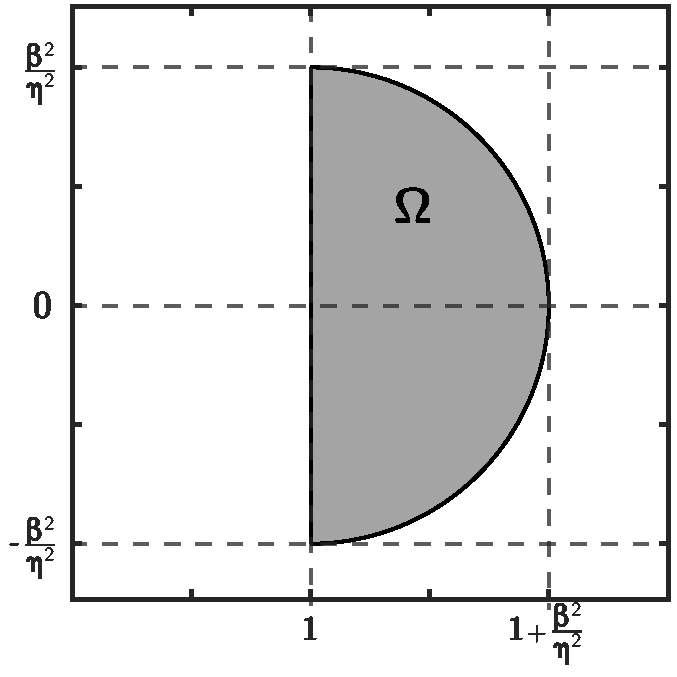
\includegraphics[width = 0.3\textwidth]{fov.pdf}
\caption{}
\label{fig:bound}
\end{figure}
\end{theorem}
\begin{proof}
For operator $M$, let $\sigma(M)$ denote the spectrum of $M$, $\sigma_{\textnormal{min}}(M)$
and $\sigma_{\textnormal{max}}(M)$ the minimum and maximum eigenvalues, and $\rho(M)$
the spectral radius. Also, define the symmetric/skew-symmetric splitting
$M = M_s + M_k$, where $M_s := (M+M^T)/2$ and $M_k := (M - M^T)/2$, and the numerical
radius as $r(M) = \sup \{ |\lambda| : \lambda \in W(M) \}$. Recall
the following properties of $W(M)$:\todo{citations}
%
\begin{enumerate}
	\item $W(M)\subset [\sigma_{\textnormal{min}}(M_s), \sigma_{\textnormal{max}}(M_s)] \times
	[-\rho(M_k)\mathrm{i}, \rho(M_k)\mathrm{i}]$.

	\item $\sigma(M) \subset W(M)$.

	% <Mv,v> + <v,Mv> > 0 ---> w = M^{-1}v ---> <w, M^{-1}w> + <M^{-1}w,w> > 0
	\item If $M$ is invertible and $M_s \leq 0$ in the symmetric negative semi-definite
	sense, then the symmetric part of $M^{-1}$ is also negative semi-definite.

	\item $r(M) \leq \|M\|_2$.

	\item $W(I + M) = 1 + W(M)$.
\end{enumerate}
%
Note that an exact inverse yields $\mathcal{P}_A = I$, with spectrum
and field-of-values given by $\sigma(\mathcal{P}_S) = W(\mathcal{P}_S) = \{1\}$.
Appealing to \eqref{eq:prec1} and the final property stated above, $W(\mathcal{P}_A)
= 1 + \tfrac{\beta^2}{\eta^2}W(E)$, for error term $E := (I - \tfrac{1}{\eta}\mathcal{L})^{-2}$
and real-valued constant $\beta^2/\eta^2 > 0$. Next we will bound $W(E)$ in the complex plane.

Assume that $\eta > 0$ and the symmetric part of $\mathcal{L}$ satisfies
$(\mathcal{L}+\mathcal{L}^T)/2 \leq 0$.
\tcb{This is somehow related/necessary to RK stability??}
It follows that the real part of eigenvalues of $\mathcal{L}$ are non-positive and,
thus, $(I - \tfrac{1}{\eta}\mathcal{L})$ cannot have a zero eigenvalue and must be
invertible. Furthermore, it also follows that the symmetric part of
$(I - \tfrac{1}{\eta}\mathcal{L})$ is symmetric positive definite and thus
the symmetric part of $(I - \tfrac{1}{\eta}\mathcal{L})^{-2}$ is as well.
This yields a lower bound of zero on the real-axis for $W(E)$, that is,
Re$(W(E)) > 0$. 

Now, note that by the assumption $(\mathcal{L}+\mathcal{L}^T)/2 \leq 0$, we have
%
\begin{align}\label{eq:norm1}
\frac{\left\langle (I - \tfrac{1}{\eta}\mathcal{L})\mathbf{x},(I - \tfrac{1}{\eta}\mathcal{L})\mathbf{x}\right\rangle}
	{\langle\mathbf{x},\mathbf{x}\rangle} 
& = 1 - \frac{\langle (\mathcal{L} + \mathcal{L}^T )
	\mathbf{x},\mathbf{x}\rangle}{\eta \langle\mathbf{x},\mathbf{x}\rangle} +
	\frac{\langle \tfrac{1}{\eta^2}\mathcal{L}^T\mathcal{L}\mathbf{x},
	\mathbf{x}\rangle}{\langle\mathbf{x},\mathbf{x}\rangle}
\geq 1
\end{align}
%
for all $\mathbf{x}\neq\mathbf{0}$. Then,
%
\begin{align*}
\|(I - \tfrac{1}{\eta}\mathcal{L})^{-2}\| \leq \|(I - \tfrac{1}{\eta}\mathcal{L})^{-1}\|^2
& = \sup_{\mathbf{x}\neq\mathbf{0}} 
	\frac{\left\langle (I - \tfrac{1}{\eta}\mathcal{L})^{-1}\mathbf{x},
	(I - \tfrac{1}{\eta}\mathcal{L})^{-1}\mathbf{x}\right\rangle}
	{\langle\mathbf{x},\mathbf{x}\rangle} \\
&\hspace{-10ex}= \sup_{\mathbf{y}\neq\mathbf{0}} 
	\frac{\langle\mathbf{y},\mathbf{y}\rangle}{\left\langle (I - \tfrac{1}{\eta}\mathcal{L})\mathbf{y},
	(I - \tfrac{1}{\eta}\mathcal{L})\mathbf{y}\right\rangle}
\leq 1.
\end{align*}
%
This yields a bound on the numerical radius $r(E) = r((I - \tfrac{1}{\eta}\mathcal{L})^{-2})
\leq \|(I - \tfrac{1}{\eta}\mathcal{L})^{-2}\|\leq 1$. Combining with Re$(W(E)) > 0$,
the field of values of the error term, $W(E)$, is contained in the positive half of the
unit circle in the complex plane, which completes the proof.
\end{proof}
%

%
\begin{corollary}\label{cor:gmres}
Let $\pi_k$ denote the set of consistent polynomials of degree $k$. Then the ideal GMRES bound
(an upper bound in operator norm on worst-case convergence) on convergence after $k$ iterations
applied to the preconditioned operator $\mathcal{P}_A$ \eqref{eq:prec1} is bounded by
\begin{align*}
\min_{p\in\pi_k} \|p(\mathcal{P}_A)\| \leq 2\left(\frac{\beta^2/\eta^2}{2 + \beta^2/\eta^2}\right)^k.
\end{align*}
\end{corollary}
\begin{proof}
For operator $M$, let $\nu(M)$ denote the distance of $W(M)$ from the origin. In \todo{cite Liesen},
they define $\cos(\beta) := \nu(M) / r(M)$, and prove that worst-case convergence of GMRES applied
to operator $M$ is bounded by (see Lemma 3.2)
%
\begin{align}\label{eq:gmres}
\min_{p\in\pi_k} \|p(M)\| \leq 2\left(\frac{1-\cos\beta}{1+\cos\beta}\right)^k.
\end{align}
%
For $M = \mathcal{P}_A$, we have $\nu(\mathcal{P}_A)= 1$ and $r(\mathcal{P}_A) \leq 1+\beta^2/\eta^2$.
Plugging into \eqref{eq:gmres} completes the proof. 
\end{proof}
%

{\color{blue}
\begin{itemize}
	\item Comment on size of $\eta$ and $\beta$ and convergence bounds for GMRES. Largest (squared)
	ratio I have seen is $\sim 4.29$ for RadauIIA(11), but another eigenvalue pair for the same
	scheme had ratio $\sim 0.04$, so the seem to even out.

	\item Is $\eta > 0$ always? Looks like it for everything I have tested, would be nice to
	say something general.. If not, need to confirm it holds for lots of standard methods.
	This is important assumption in above analysis.

	\item Classical GMRES convergence results based on $\lambda_{\textnormal{min}}((\mathcal{P}_A+
	\mathcal{P}_A^T)/2)$ and $\lambda_{\textnormal{max}}(\mathcal{P}_A^T\mathcal{P}_A)$ can also
	be applied, yielding a less tight result of $\left(\frac{\beta^2/\eta^2}{1 + \beta^2/\eta^2}\right)^{k/2}$.
	The field-of-values is $2-4\times$ tighter, and deriving the field-of-values also reflects the
	nice conditioning of the operator. 

\end{itemize}
}

% ----------------------------------------------------------------------------------------------------------- %
% ----------------------------------------------------------------------------------------------------------- %
\subsection{Preconditioning quadratic polynomials}

In practice, we generally do not want to directly form preconditioners for a quadratic
polynomial in $\mathcal{L}$. Even forming such an operator can be expensive in parallel.
Moreover, many well-known fast parallel preconditioners such as multigrid would likely
struggle when applied directly to a matrix quadratic. Instead, the previous section
suggests we can use two successive applications of a preconditioner for
$(\eta I - \mathcal{L})$. If $(\eta I - \mathcal{L})^{-1}$
is applied twice to the \textit{action} of $(\eta^2+\beta^2)I - 2\eta\mathcal{L} + \mathcal{L}^2$,
\Cref{th:fov} proves that the preconditioned operator is very well conditioned and GMRES
will converge rapidly (see also \Cref{cor:gmres}). However, in practice, fully converging
$(\eta I - \mathcal{L})^{-1}$ is not desirable --  even if GMRES converges rapidly,
if each iteration requires a full linear solve, the resulting method remains moderately
expensive. 
Here, we propose applying GMRES to $(\eta^2+\beta^2)I - 2\eta\mathcal{L} + \mathcal{L}^2$
by computing the operator's action (that is, not fully constructing it), and preconditioning
each GMRES iterations with \textit{two} applications of a sparse parallel preconditioner for
$(\eta I - \mathcal{L})$, representing the action of $(\eta I - \mathcal{L})^{-2}$. 



{\color{blue}
\begin{itemize}
	\item I am thinking each GMRES iteration we only do a few (or even one?) AMG iterations
	for each application of $(\alpha I - \mathcal{L})$, hoping that at the end it doesn't
	really take more iterations than if we were to directly apply AMG preconditioned GMRES
	to $(\alpha I - \mathcal{L})^2$.

	\item We are actually preconditioning a much worse-conditioned operator. The $+\beta^2$
	term we get in the operator (rather than preconditioner) shifts the field-of-values 
	positive and away from the origin by $\beta$. Hopefully this pans out by observing
	rapid convergence..

	\item One thing I am really puzzled by -- by formulating based on $A_0^{-1}$, the
	eigenvalues in my tests appear to be fairly large in magnitude. E.g., eigenvalues of
	$A_0$ are $\sim 0.1$ and eigenvalues of $A_0^{-1}$ are $\sim 5$. If this is true and we
	can get away with solving $(\eta I -\mathcal{L})$ for $\eta \sim 10\times$ larger than
	eigenvalues of $A_0$, that could be huge. In theory such systems would likely be way
	better conditioned. It also seems too good to be true/not very intuitive to solve a
	system with such a big shift when our actual time step is $\ll$..

\end{itemize}
}




% ------------------------------------------------------------------------------- %
% \bibliographystyle{siamplain}
% \bibliography{refs.bib}


\end{document}
